\documentclass[10pt,xcolor=pdflatex,hyperref={unicode,hidelinks}]{beamer}

\usepackage{newcent}
\usepackage[utf8]{inputenc}
\usepackage[T1]{fontenc}
\usepackage[czech]{babel}
\usepackage{amsmath,amsfonts,amssymb}
\usepackage{fancyvrb}
\usepackage{url}
\usepackage{algorithmicx}
\usepackage[noend]{algpseudocode}
\usetheme{FIT}

\usepackage{tikz}

\usetikzlibrary{graphs,graphs.standard,arrows.meta,automata,positioning,quotes}

\deftranslation[to=czech]{Definition}{Definice}

\title[IVS -- projekt 2]{IVS projekt: Kalkulačka SunnyCalc}

\author[]{Pracovní skupina Sluníčka}

\institute[]{Fakulta informačních technologií VUT v Brně\\
Bo\v{z}et\v{e}chova 1/2, 612 00 Brno-Kr\'alovo Pole}

\date{\today}

\begin{document}

\frame[plain]{\titlepage}

\begin{frame}{Produkt}
\begin{columns}[T]
    \column{0.6\textwidth}
    \begin{itemize}
        \item Kalkulačka se základním a~rozšířeným módem
        \begin{itemize}
            \item Základní operace (+,-,*,/)
            \item Umocňování, odmocňování s~obecným exponentem
            \item Goniometrické funkce
            \item Faktoriál
        \end{itemize}
        \item Vyhodnocování komplexních výrazů se závorkami
        \item Integrovaná nápověda a~uživatelská dokumentace
    \end{itemize}
    \column{0.4\textwidth}
    \centering
    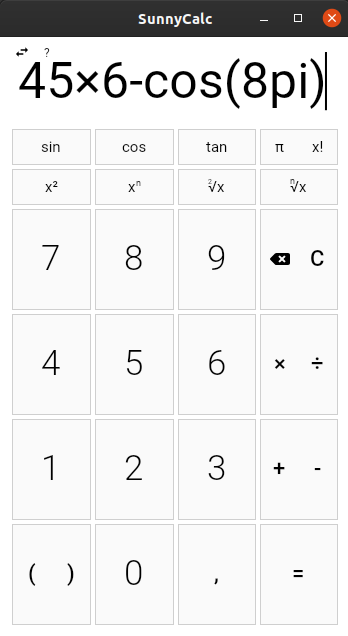
\includegraphics[height=0.85\textheight]{img/sunnyc.png}
\end{columns}
\end{frame}

\begin{frame}{Produkt -- technologie}
    \begin{itemize}
        \item Platforma: .NET Core 3.1
        \item Jazyk: C\#
        \item GUI framework: Avalonia
        \item Licence: Open-source (GNU GPL 3)
        \item Multiplatformní
    \end{itemize}
\end{frame}

\begin{frame}{Použité nástroje}
    \begin{itemize}
        \item Verzování, issue tracking, code review: GitHub
        \item Continuous integration: Travis CI
        \item Vývojové prostředí: JetBrains Rider + dotTrace (profiling)
        \item Instalátor (Windows): InnoSetup
        \item Balíčkovací toolset Debianu
        \item Doxygen, GNU Make
    \end{itemize}
\end{frame}

\begin{frame}{Zkušenosti -- verzování}
    \begin{itemize}
        \item<only@1,4,6-> Struktura repozitáře
        \item<only@1,4,6-> Feature branches
        \item<only@1,4,6-> Pull requesty a code review
        \item<only@4,6-> Issue tracking
        \item<only@6-> Integrace GitHubu a Travis CI
        \item<only@6-> Merging, rebasing, cherry-pick
    \end{itemize}
    \only<2>{
        \centering
        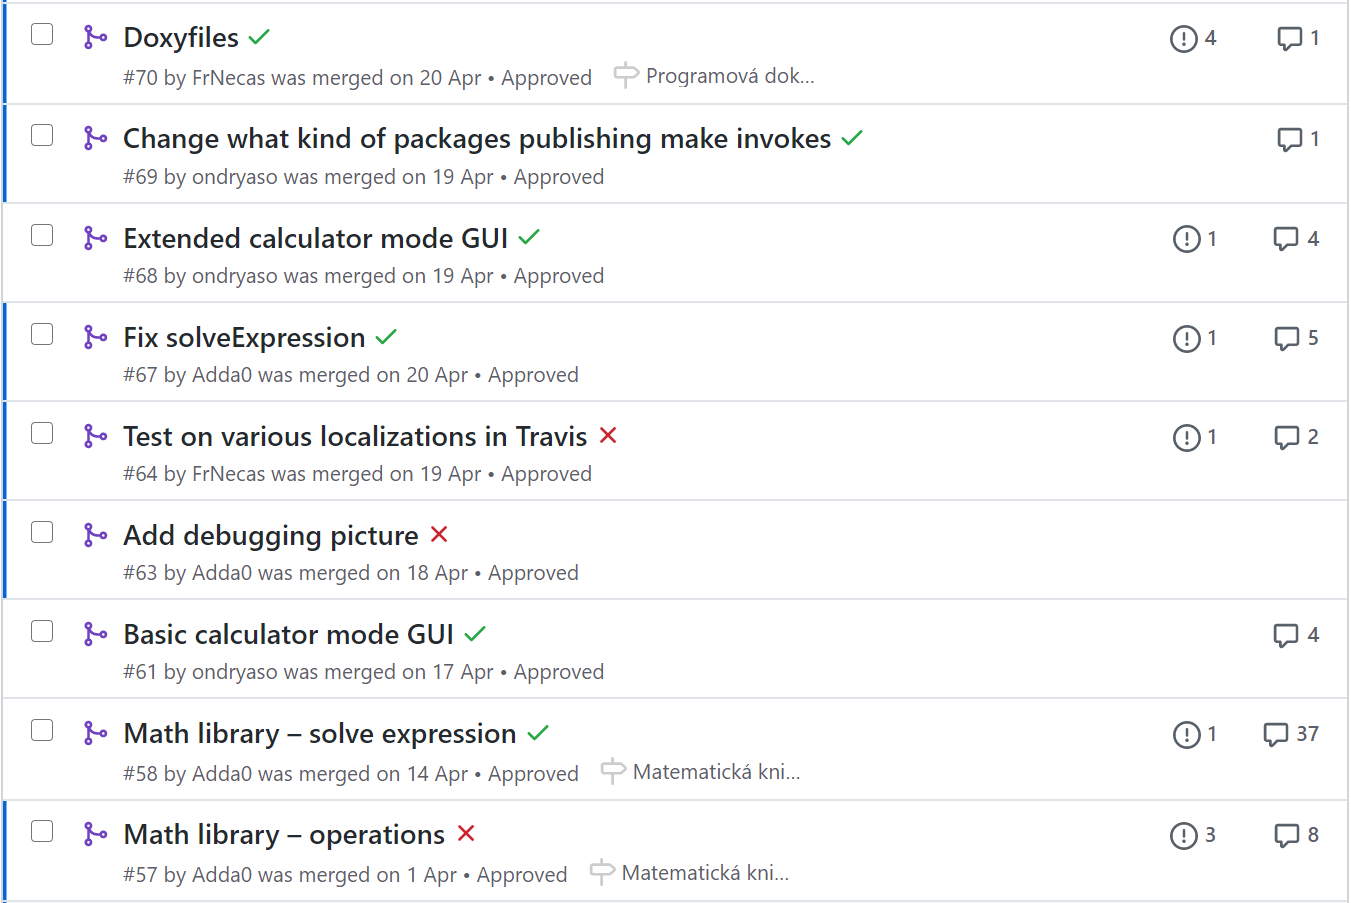
\includegraphics[width=\framewidth]{img/PR.png}
    }
    
    \only<3>{
        \centering
        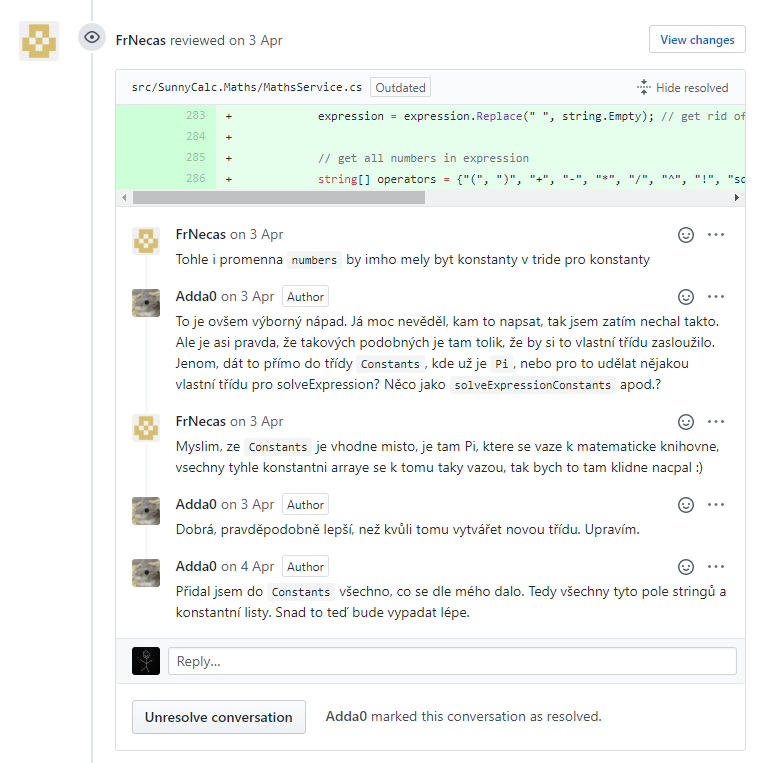
\includegraphics[height=0.85\textheight]{img/PR_disc.png}
    }
    
    \only<5>{
         \centering
        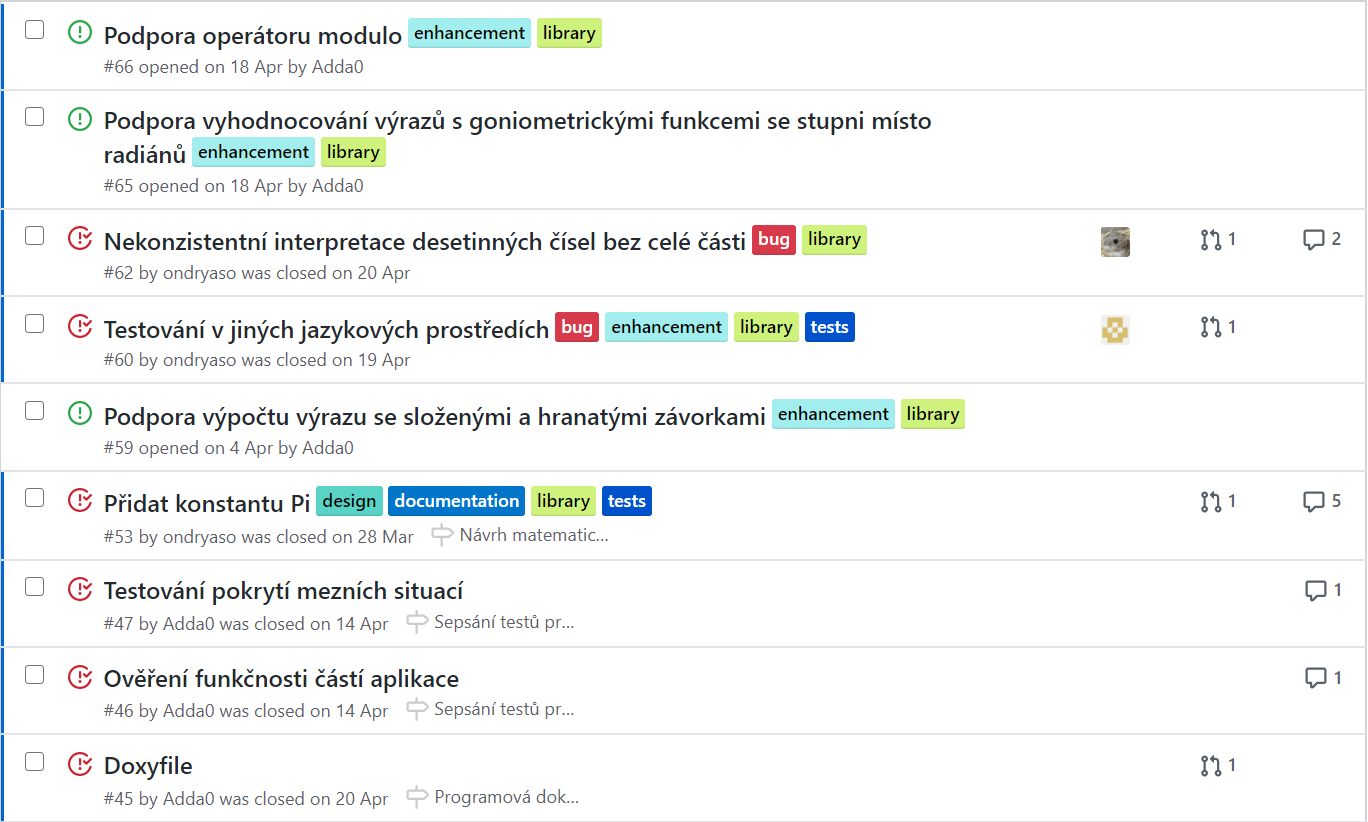
\includegraphics[width=\framewidth]{img/Issues.png}
    }
\end{frame}

\begin{frame}{Zkušenosti -- spolupráce v týmu}
    \begin{itemize}
        \item<only@1,3-> Komunikační kanál: Discord, GitHub
        \item<only@3-> Lehký časový skluz, ale v plánu byly rezervy
        \item<only@3-> Zodpovědnost
    \end{itemize}
    
    \only<2>{
        \centering
        
\includegraphics[height=0.85\textheight]{img/discord.png}
    }
\end{frame}

\begin{frame}\frametitle{Tým}
    \renewcommand\UrlFont{\ttfamily\footnotesize}
    \begin{itemize}
        \item František Nečas (xnecas27)
        \item Ondřej Ondryáš (xondry02)
        \item David Chocholatý (xchoch08)
    \end{itemize}
\end{frame}

\bluepage{Děkujeme za pozornost.}


\end{document}
